\documentclass{standalone}
\usepackage{tikz}
\usetikzlibrary{shapes.geometric, shapes.misc, arrows.meta, calc, backgrounds, decorations.markings}

%% ── Hop-over decoration ─────────────────────────────────────────────────────
%% Draws a small semicircular bump at the midpoint of a path segment to
%% indicate that two lines cross without connecting.
\tikzset{
    hopon/.style={
        postaction={decorate,
            decoration={markings,
                mark=at position 0.5 with {
                    \draw[line width=1pt, fill=white]
                        (-2pt,0) arc[start angle=180, end angle=0, radius=2pt];
                }
            }
        }
    },
}

\begin{document}
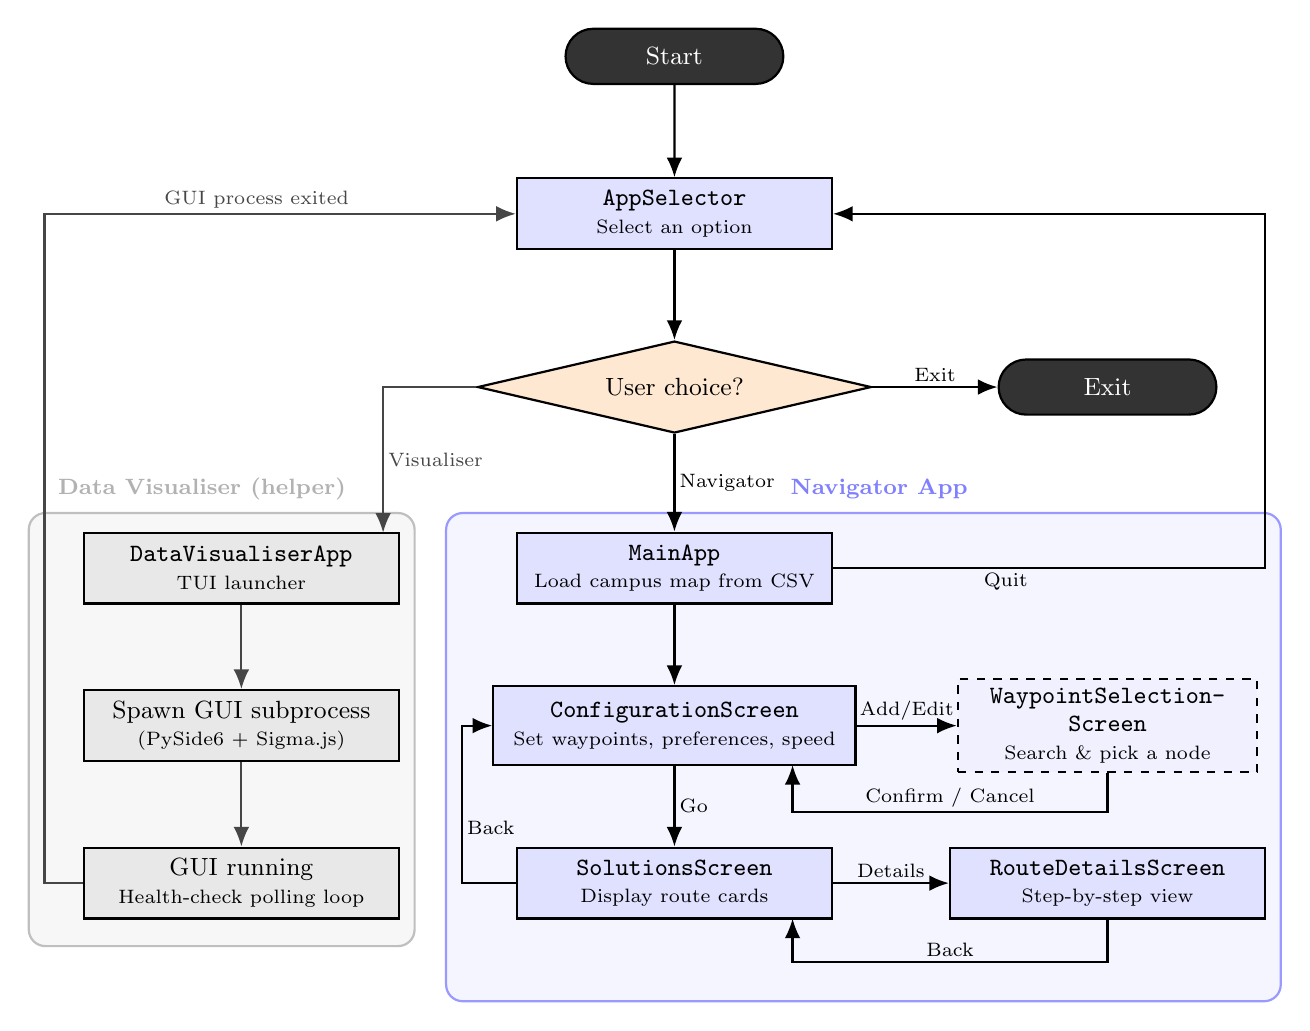
\begin{tikzpicture}[
    font=\small,
    arr/.style={-{Latex[length=2.5mm, width=2mm]}, thick},
    arrv/.style={-{Latex[length=2.5mm, width=2mm]}, thick, gray!55!black},
    lbl/.style={font=\scriptsize, inner sep=1.5pt},
]

%% ═══════════════════════════════════════════════════════════════════════════
%% COORDINATE GRID  (all lengths in cm)
%%
%%   x = 0.0   Visualiser column (left)
%%   x = 5.5   Main spine / Navigator column (centre)
%%   x = 11.0  Modal / side-screen column (right)
%%
%%   y = 0.0   Start
%%   y = -2.0  AppSelector box
%%   y = -4.2  Decision diamond
%%   y = -6.5  MainApp  |  DataVisualiserApp
%%   y = -8.5  ConfigurationScreen
%%   y = -10.5 SolutionsScreen
%%   y = -12.5 RouteDetailsScreen
%%   y = -14.8 (loop-back anchor below RouteDetails)
%% ═══════════════════════════════════════════════════════════════════════════

%% ── Nodes ──────────────────────────────────────────────────────────────────

%% Start / End terminals  (pill shape)
\node[draw, thick, fill=black!80, text=white,
      rounded rectangle, rounded rectangle arc length=180,
      minimum width=3.0cm, minimum height=0.7cm]
    (start) at (5.5, 0) {Start};

\node[draw, thick, fill=black!80, text=white,
      rounded rectangle, rounded rectangle arc length=180,
      minimum width=3.0cm, minimum height=0.7cm]
    (exitnode) at (11, -4.2) {Exit};

%% AppSelector
\node[draw, thick, fill=blue!12, rectangle,
      minimum width=4.0cm, minimum height=0.9cm, align=center]
    (selector) at (5.5, -2.0)
    {\texttt{AppSelector}\\[-1pt]\scriptsize Select an option};

%% Choice diamond
\node[draw, thick, fill=orange!18, diamond, aspect=2.8,
      minimum width=5.0cm, minimum height=1.0cm, align=center]
    (choice) at (5.5, -4.2) {User choice?};

%% ─── Navigator branch ──────────────────────────────────────────────────────
\node[draw, thick, fill=blue!12, rectangle,
      minimum width=4.0cm, minimum height=0.9cm, align=center]
    (mainapp) at (5.5, -6.5)
    {\texttt{MainApp}\\[-1pt]\scriptsize Load campus map from CSV};

\node[draw, thick, fill=blue!12, rectangle,
      minimum width=4.6cm, minimum height=1.0cm, align=center]
    (config) at (5.5, -8.5)
    {\texttt{ConfigurationScreen}\\[-1pt]\scriptsize Set waypoints, preferences, speed};

\node[draw, thick, fill=blue!6, dashed, rectangle,
      minimum width=3.8cm, minimum height=1.0cm, align=center]
    (wpsel) at (11.0, -8.5)
    {\texttt{WaypointSelection-}\\[-1pt]\texttt{Screen}\\[-1pt]\scriptsize Search \& pick a node};

\node[draw, thick, fill=blue!12, rectangle,
      minimum width=4.0cm, minimum height=0.9cm, align=center]
    (solutions) at (5.5, -10.5)
    {\texttt{SolutionsScreen}\\[-1pt]\scriptsize Display route cards};

\node[draw, thick, fill=blue!12, rectangle,
      minimum width=4.0cm, minimum height=0.9cm, align=center]
    (details) at (11.0, -10.5)
    {\texttt{RouteDetailsScreen}\\[-1pt]\scriptsize Step-by-step view};

%% ─── Visualiser branch ─────────────────────────────────────────────────────
\node[draw, thick, fill=gray!18, rectangle,
      minimum width=4.0cm, minimum height=0.9cm, align=center]
    (visapp) at (0.0, -6.5)
    {\texttt{DataVisualiserApp}\\[-1pt]\scriptsize TUI launcher};

\node[draw, thick, fill=gray!18, rectangle,
      minimum width=4.0cm, minimum height=0.9cm, align=center]
    (guiproc) at (0.0, -8.5)
    {Spawn GUI subprocess\\[-1pt]\scriptsize (PySide6 + Sigma.js)};

\node[draw, thick, fill=gray!18, rectangle,
      minimum width=4.0cm, minimum height=0.9cm, align=center]
    (visrunning) at (0.0, -10.5)
    {GUI running\\[-1pt]\scriptsize Health-check polling loop};

%% ═══════════════════════════════════════════════════════════════════════════
%% ARROWS
%% ═══════════════════════════════════════════════════════════════════════════

%% Start → AppSelector
\draw[arr] (start) -- (selector);

%% AppSelector → choice diamond
\draw[arr] (selector) -- (choice);

%% choice → Exit  (east, horizontal)
\draw[arr] (choice.east) -- (exitnode.west)
    node[lbl, midway, above] {Exit};

%% choice → MainApp  (south, vertical)
\draw[arr] (choice.south) -- (mainapp.north)
    node[lbl, midway, right] {Navigator};

%% choice → DataVisualiserApp
\draw[arrv] (choice.west) -- (1.8, -4.2) -- (1.8, -6.05) node[lbl, midway, right] {Visualiser};

%% ─── Navigator flow ────────────────────────────────────────────────────────

%% MainApp → ConfigurationScreen
\draw[arr] (mainapp) -- (config);

%% ConfigurationScreen → WaypointSelectionScreen
%%   east from config → wpsel west
\draw[arr] (config.east) -- (wpsel.west)
    node[lbl, midway, above] {Add/Edit};

%% WaypointSelectionScreen → back to ConfigurationScreen
%%   from wpsel.south, drop to y=-9.4, go left to x=5.5+2.3=7.8, then into config.east
\draw[arr]
    (wpsel.south) -- (11.0, -9.6) -- (7, -9.6)
    node[lbl, midway, above] {Confirm / Cancel} -- (7, -9);

%% ConfigurationScreen → SolutionsScreen  (Go button)
\draw[arr] (config.south) -- (solutions.north)
    node[lbl, midway, right] {Go};

%% SolutionsScreen → RouteDetailsScreen  (east)
\draw[arr] (solutions.east) -- (details.west)
    node[lbl, midway, above] {Details};

%% RouteDetailsScreen → SolutionsScreen  (back)
%%   from details.south drop to y=-11.4, left to x=7.8, up into solutions.east
\draw[arr]
    (details.south) -- (11.0, -11.5) -- (7, -11.5)
    node[lbl, midway, above] {Back} -- (7, -10.95);

%% SolutionsScreen → ConfigurationScreen  (Back / Escape)
%%   Left side: from solutions.west x=3.3, down to y=-12.0, left to x=3.0,
%%   up to y=-8.5, into config.west
\draw[arr]
    (solutions.west) -- (2.8, -10.5) -- node[lbl, pos=0.35, right] {Back} (2.8, -8.5) -- (config.west);

%% MainApp → AppSelector  (Ctrl+Q — quit)
%%   Right side spine: from mainapp.east x=7.5, right to x=8.5,
%%   up to y=-2.0, into selector.east
\draw[arr]
    (mainapp.east) -- (13.0, -6.5) node[lbl, pos=0.4, below] {Quit} -- (13.0, -2.0) -- (selector.east);

%% ─── Visualiser flow ────────────────────────────────────────────────────────
\draw[arrv] (visapp) -- (guiproc);
\draw[arrv] (guiproc) -- (visrunning);

% %% Polling loop (self-loop on right side of visrunning)
% \draw[arrv]
%     (visrunning.east) -- (1.8, -10.5) -- (1.8, -9.5)
%     node[lbl, midway, right] {Still running}
%     -- (1.8, -8.5) -- (guiproc.east);

%% GUI closed → back to AppSelector
%%   from visrunning.west, left to x=-2.5, up to y=-2.0, into selector.west
\draw[arrv]
    (visrunning.west) -- (-2.5, -10.5) -- (-2.5, -2.0) -- (selector.west)
    node[lbl, pos=0.45, above] {GUI process exited};

%% ═══════════════════════════════════════════════════════════════════════════
%% BACKGROUND PANELS
%% ═══════════════════════════════════════════════════════════════════════════
\begin{scope}[on background layer]
    \filldraw[draw=blue!40, fill=blue!4, thick, rounded corners=6pt]
        (2.6, -5.8) rectangle (13.2, -12.0);
    \node[blue!50, font=\footnotesize\bfseries] at (8.1, -5.5) {Navigator App};

    \filldraw[draw=gray!50, fill=gray!6, thick, rounded corners=6pt]
        (-2.7, -5.8) rectangle (2.2, -11.3);
    \node[gray!60, font=\footnotesize\bfseries] at (-0.5, -5.5) {Data Visualiser (helper)};
\end{scope}

\end{tikzpicture}
\end{document}
